\section{Additional Details on Agentic Tasks}
\label{appendix:detail_application}


\subsection{Experience Bank and Training Data Construction}

\subsubsection{Experience Bank Construction}

We construct the experience bank in four stages. First, we treat each trajectory as an episode and annotate it with its key decisions and a state signature comprising topic tags, the first tool used, and the error code. Second, episodes with the same state signature are pooled, and DeepSeek-V4-Pro~\cite{deepseekai2026deepseekv4} induces a policy of the form ``when condition \(X\) holds, take action \(Y\), verify with \(Z\), and watch out for \(W\)'' from each pool. Each policy must specify a trigger observable from the agent's state. Source-specific entities such as repository, product, and file names are abstracted into variables. Third, policies describing the same workflow are clustered based on the lexical similarity of their titles, triggers, and procedures, with one policy retained as the representative of each cluster. Finally, DeepSeek-V4-Pro synthesizes a structured experience from the trajectories supporting each representative policy. An automated check verifies that the declared tools appear in the supporting trajectories, and a separate LLM audit
filters out experiences containing severe errors.

We summarize the construction funnel and the
resulting experience bank in Table~\ref{tab:experience-bank}. Each experience contains ten fields, including a retrieval description to support matching, a trigger context specifying when it applies, steps and parameters specifying what to do, preconditions defining its scope of applicability, and decision guidance documenting preferred choices and potential pitfalls.

Most experiences are specific, since 942 of the 1{,}040 derive from a single trajectory, while a few broad workflows draw on hundreds. The bank emphasizes procedural guidance and verification, with verification and testing-related tags among the most frequent after the python tag. Issue-level retrieval provides limited discrimination among top-ranked candidates: the median difference in similarity scores between the first- and fifth-ranked candidates is only 0.029.

\begin{table}[htbp]
  \centering
  \caption{Experience bank construction and statistics. Token
  counts use the Qwen3.6-35B-A3B tokenizer.}
  \label{tab:experience-bank}
  \small
  \begin{adjustbox}{max width=\linewidth}
  \begin{tabular}{lr}
    \toprule
    \multicolumn{2}{l}{(a) Construction stages}\\
    \midrule
    Source trajectories (23{,}667 instances, 2{,}562 repositories) & 41{,}057\\
    Induced policies (88.5\% cite a single trajectory) & 3{,}678\\
    Representative policies after clustering & 1{,}200\\
    Audit: usable / usable with caveat / severe error & 401 / 639 / 160\\
    \textbf{Experiences in the final bank} & \textbf{1{,}040}\\
    \midrule
    \multicolumn{2}{l}{(b) Bank statistics}\\
    \midrule
    Fields per experience & 10\\
    Length as JSON / as rendered text (tokens, mean) & 715 / 456\\
    Rendered text, 10th / 90th percentile (tokens) & 391 / 521\\
    Steps per experience (range; experiences with five steps) & 3--6; 573\\
    Source trajectories per experience (mean; single-source experiences) & 3.0; 942\\
    Most frequent tags: \emph{python} / \emph{verification} / \emph{testing} / \emph{pytest} & 792 / 192 / 168 / 133\\
    Top-1 cosine similarity (mean; 10th--90th percentile) & 0.611; 0.556--0.668\\
    Median similarity gap between top-1 and top-5 & 0.029\\
    \bottomrule
  \end{tabular}
  \end{adjustbox}
\end{table}

\subsubsection{Experience-Conditioned Trajectory Construction}

We construct experience-conditioned training trajectories in five stages, as demonstrated in Figure~\ref{fig:data-construction-pipeline}: generating original trajectories, identifying candidate breakpoints, selecting and injecting experiences, validating the intervention outcomes, and serializing the resulting training examples.

We represent an agent trajectory as
\[
    \xi =
    \left(
        h_0, a_0, o_0,
        \ldots,
        h_T, a_T, o_T
    \right),
\]
where \(h_t\), \(a_t\), and \(o_t\) denote the interaction history before step \(t\), the action produced by the agent, and the corresponding environment observation, respectively.

\begin{figure}[tb]
    \centering
    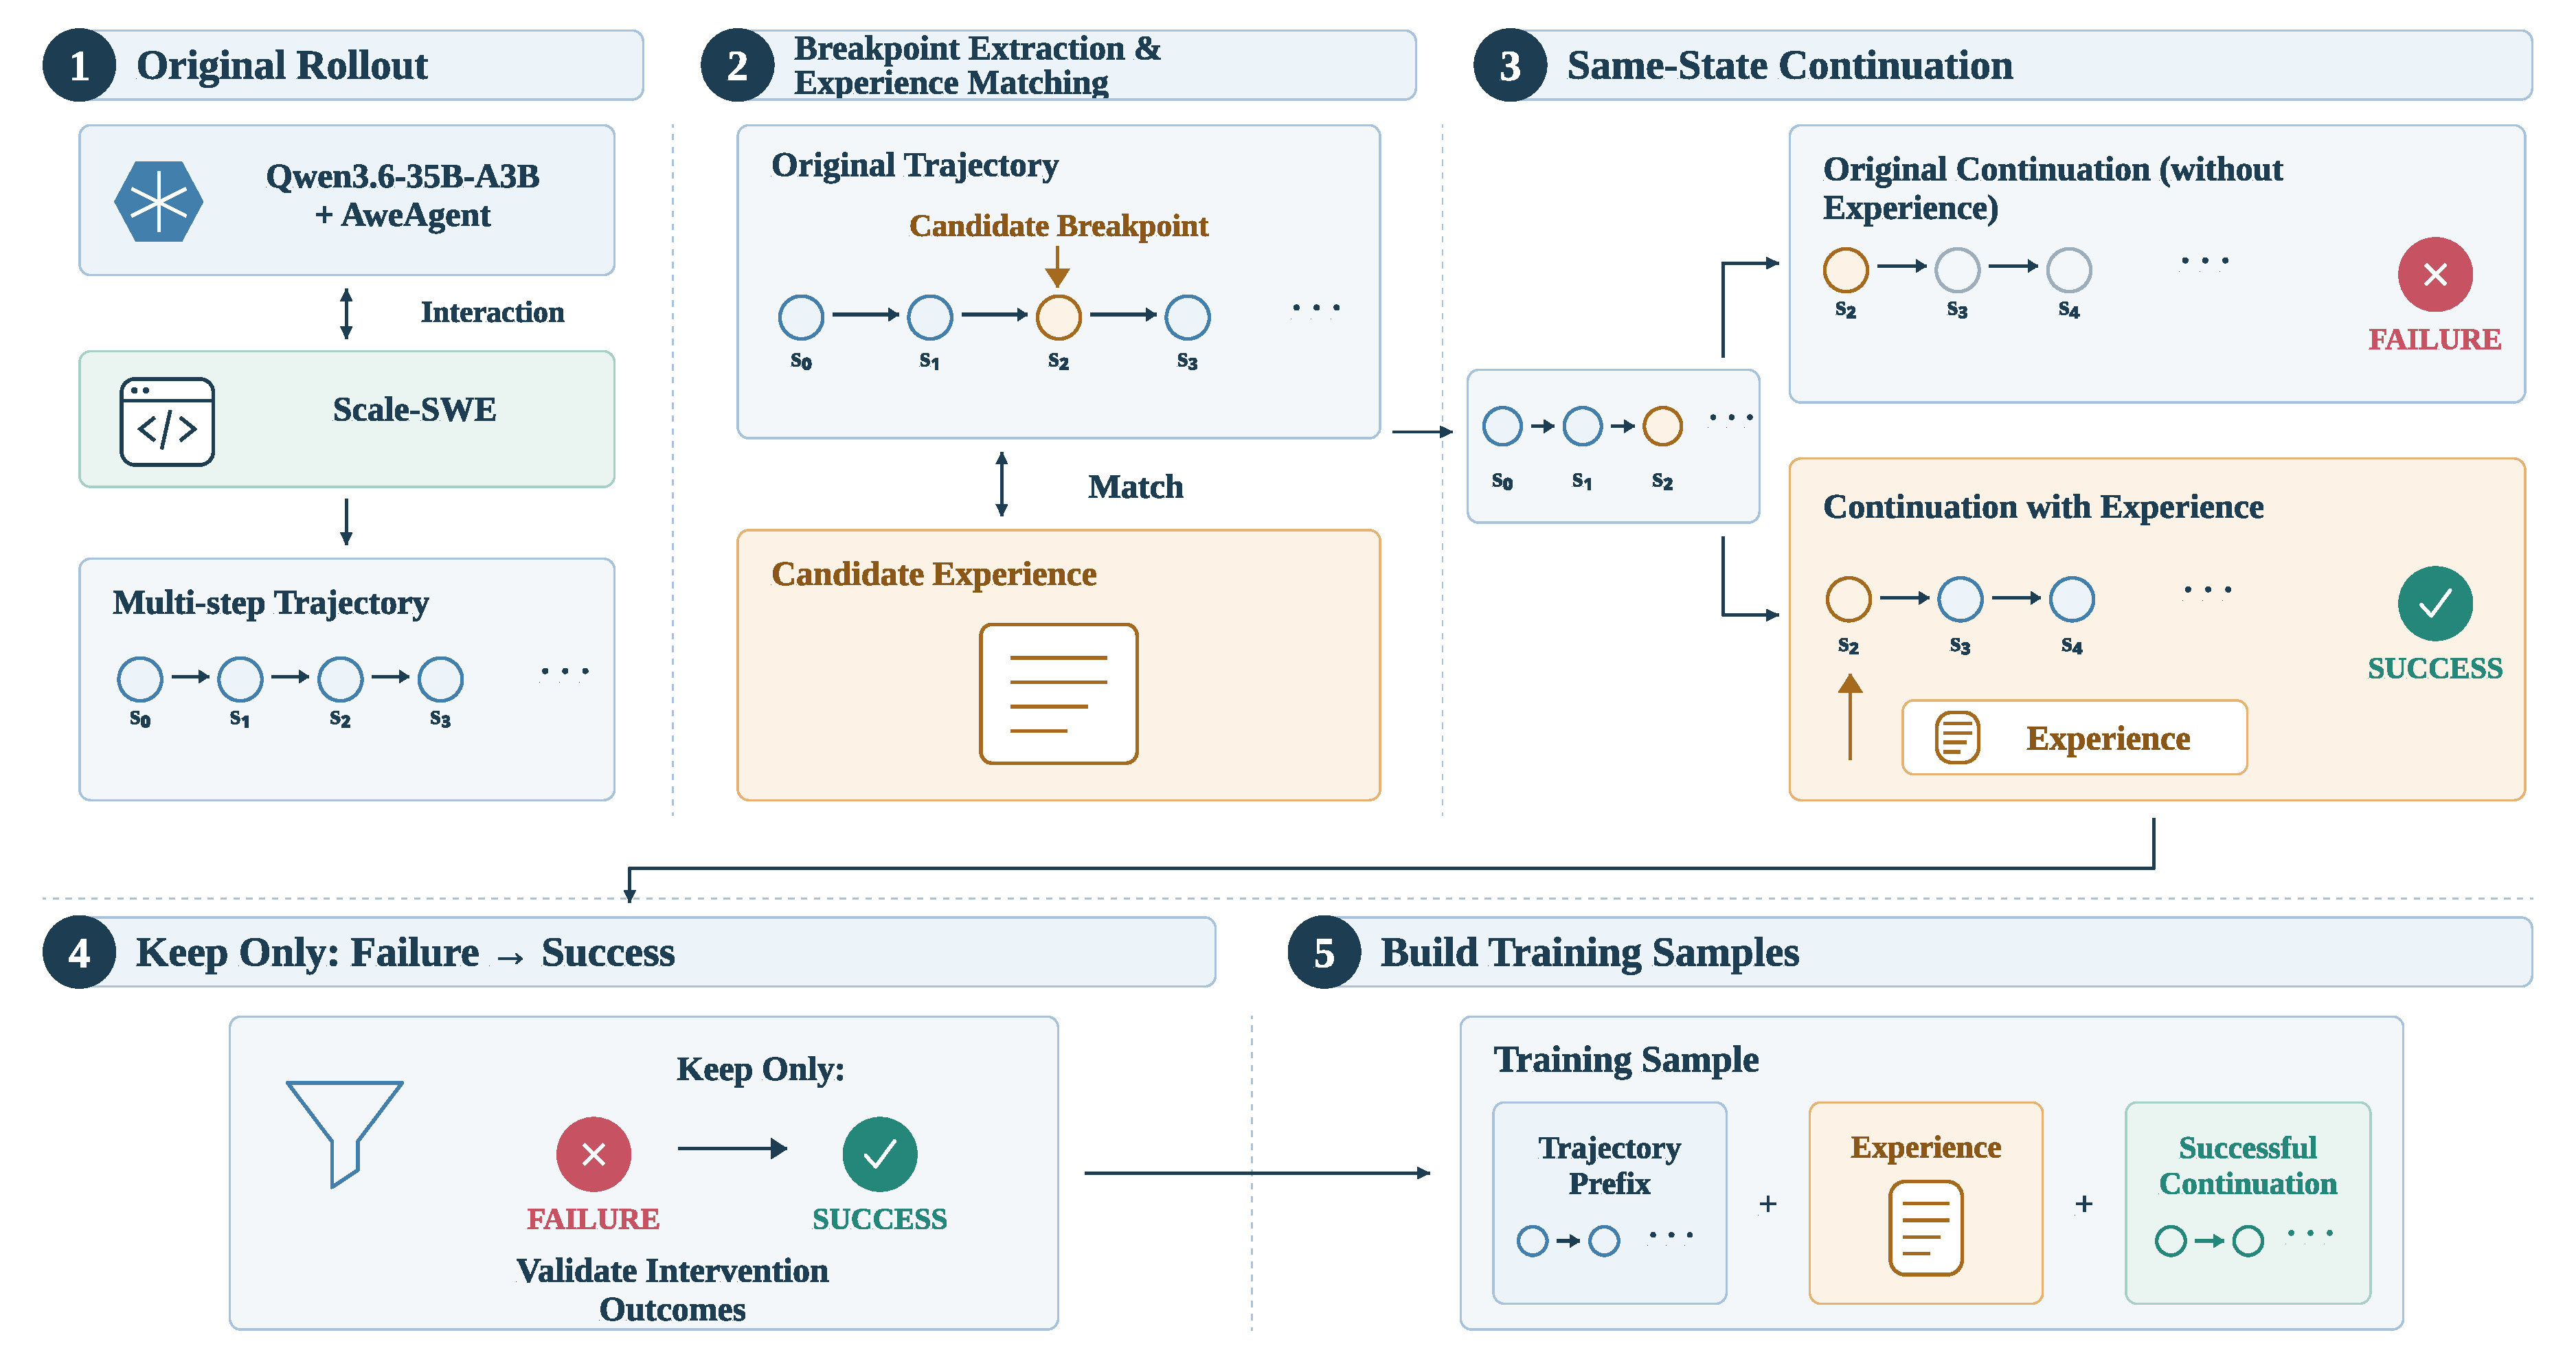
\includegraphics[width=\linewidth]{figures/application/training_data_construction.pdf}
    \caption{Construction of experience-conditioned training trajectories. Retrieved experience is added at selected breakpoints in unsuccessful trajectories, and execution resumes from the same state. Continuations that pass the task tests are retained as training samples comprising the trajectory prefix, experience, and successful continuation.}
    \label{fig:data-construction-pipeline}
\end{figure}

\paragraph{Breakpoint Identification}
\label{subsec:breakpoint-extraction}

For unsuccessful trajectories, we sequentially scan the observations in each rollout. A step $t$ is marked as a candidate breakpoint based on execution feedback, including command failures, empty observations after normalization, and repeated unsuccessful operations. This criterion relies only on feedback visible to the agent at execution time and does not access reference solutions or privileged evaluation information.

To prevent long trajectories from producing a disproportionate number of intervention variants, we retain at most eight breakpoints per rollout. If a rollout contains more than eight candidates, we sample eight of them without replacement using a fixed random seed. We additionally record the total number of candidate breakpoints and the positions of the retained breakpoints to ensure reproducibility. The Harness-Triggered evaluation setting uses the same breakpoint-detection logic, with at most one experience store operation per trajectory. Before Execution evaluates robustness to experience injection timing.

\paragraph{Experience Retrieval and Counterfactual Validation}
\label{subsec:experience-validation}

For each task, we first retrieve the top-10 most relevant entries from the experience bank. We then construct ten candidate experience subsets for every retained breakpoint: one subset containing the complete top-3 entries, one containing the complete top-5 entries, and eight three-entry subsets sampled from the top-10 retrieved entries. Random sampling is performed using a fixed seed associated with each task instance.

Each breakpoint-experience-subset pair defines an independent continuation rollout. The resulting intervention trajectory is
\[
    \xi_{b,j}
    =
    \xi_{\leq b}
    \oplus
    [g_{b,j}]
    \oplus
    \hat{\xi}_{>b}^{(g_{b,j})}.
\]
Here, $b$ indexes the selected breakpoint, $j$ indexes the candidate experience subset, and \(\oplus\) denotes concatenation of message sequences. We retain a trajectory as a training sample if and only if
\[
    \begin{cases}
        \operatorname{Success}(\xi) = 0, \\
        \operatorname{Success}(\xi_{b,j}) = 1,
    \end{cases}
\]
which means the original trajectory must fail to solve the task, whereas the experience-conditioned continuation must pass the task tests. Variants that fail the tests, terminate abnormally, or cannot be reproduced are excluded from the training set.

\paragraph{Training Sample Serialization}
\label{subsec:training-example-serialization}

Finally, each training sample is serialized as
\[
    x_{b,j}
    =
    \left(
        \xi_{\leq b},
        g_{b,j},
        \hat{\xi}_{>b}^{+\left(g_{b,j}\right)}
    \right),
\]
where the three components correspond to the triggering execution state, the experience subset, and the successful continuation suffix, respectively. The superscript \(+\) indicates that the generated suffix passes the task evaluation.


\subsubsection{Dataset Statistics and Splits}

We partition the constructed data into training and validation sets by
task, keeping all original rollouts, breakpoints, and intervention
variants associated with each task in the same split, and SWE-bench Verified
serves as the test set. We report the number of tasks and repositories of each split in Table~\ref{tab:data-splits}.

\begin{table}[tb]
    \centering
    \caption{Task and repository counts for the training and validation splits and SWE-bench Verified.}
    \label{tab:data-splits}
    \begin{tabular}{lrrr}
        \toprule
        \textbf{Statistic} &
        \textbf{Train} &
        \textbf{Validation} &
        \textbf{Test (Verified)} \\
        \midrule
        Number of repositories & 537   & 176 & 12  \\
        Number of tasks        & 2,396 & 266 & 500 \\
        \bottomrule
    \end{tabular}
\end{table}

Throughout data construction, we check breakpoint validity, consistency
between trajectory prefixes and repository snapshots, test outcomes,
message and tool-call structure, and context length. We exclude samples
with environment failures, incomplete logs, test-file modifications,
other invalid execution behaviors, or outcomes that cannot be
reproduced. Samples that exceed the context-length limit or fail
structural checks are discarded in full rather than truncated. The scale of the resulting data construction process and the outcomes of experience intervention are reported in Table~\ref{tab:construction-statistics}.

\begin{table*}[tb]
    \centering
    \caption{Training data construction statistics and experience intervention outcomes.}
    \label{tab:construction-statistics}
    \begin{tabular}{p{0.31\textwidth} r p{0.47\textwidth}}
        \toprule
        \textbf{Statistic} &
        \textbf{Value} &
        \textbf{Calculation or description} \\
        \midrule
        Original trajectories
        &
        18,820
        &
        Target rollouts generated by Qwen3.6-35B-A3B
        \\

        Unsolved original trajectories
        &
        14,649 (77.8\%)
        &
        \(14{,}649 / 18{,}820\)
        \\

        Breakpoint--experience variants
        &
        199,500
        &
        7,901 usable trajectories produced 19,950 retained breakpoints
        \\

        Successful experience
        &
        45,481 (22.8\%)
        &
        \(45{,}481 / 199{,}500\)
        \\
        \bottomrule
    \end{tabular}
\end{table*}

\subsection{Training Details}

We compare training configurations along three dimensions: the objective (CE or KD), the supervision scope (First-Step or Full-Suffix), and the number of successful training trajectories selected per task. Max-2 and Max-3 retain at most two and three successful training trajectories per task, respectively.

\subsubsection{Trainable Parameters and Memory Operations}

We train Metis on hyper memory blocks at decoder layers
$\ell \in \{3, 7, 11, 15, 19, 23, 27, 31, 35, 39\}$. Each block contains 10
 trainable tensors: \text{W\_k.weight}, \text{W\_v.weight},
\text{pool\_score.weight}, \text{gated\_delta\_alpha.weight},
\text{gated\_delta\_alpha.bias}, \text{gated\_delta\_beta.weight},
\text{gated\_delta\_beta.bias}, \text{query\_proj.weight},
\text{query\_norm.weight}, and \text{mem\_norm.weight}. This gives 100
tensors and 104,962,580 trainable parameters in total, roughly 0.3\% of
the backbone's parameter count. The backbone runs in BF16, whereas the
memory computation, state accumulation, and all trainable
parameters are kept in FP32.

Each memory block maintains a fixed-size memory consisting of a
$512 \times 512$ value state and a $512 \times 1$ key normalizer, so the
memory footprint does not grow with the length of the experience. The key
and value projections map the hidden states of the experience to
512-dimensional vectors, while the query projection maps the hidden states
of the main trajectory to memory queries. On the write side, the token selector applies alpha top-$p$ selection with
$p = 0.9$ and always retains at least one token; the delta update ratio is
set to 0.9. On the read side, the memory readout is normalized by
\texttt{mem\_norm} and fused with the backbone representation using a
fusion coefficient of $\gamma = 0.9$. Runtime memory is not retained across tasks. The checkpoint contains only the
trainable memory parameters listed above, and every new task or
trajectory starts from an empty memory state.

\subsubsection{Sample Serialization and Supervision Masks}

Each training sample corresponds to exactly one write event, and the
memory is reset to empty at the start of every sample. Within a sample,
tokens are split into two attention domains: the \texttt{experience}
domain, which contains the experience text, and the \texttt{main} domain,
which contains the trajectory prefix and the successful continuation. The
\texttt{main} domain does not attend to the \texttt{experience} domain, so
the experience can influence the main trajectory only through memory.

Replay then proceeds in three stages, which mirror the injection of
experience at an execution breakpoint:
(1) \emph{write}: the experience is stored in memory at the end of the
experience segment;
(2) \emph{prefix replay}: the main-trajectory prefix is processed with
memory reading disabled; and
(3) \emph{continuation replay}: memory reading is enabled from the
breakpoint onward, so that all subsequent predictions can access the
experience-derived state $M$. Consequently, the prediction of the first supervised token is already
conditioned on the stored memory. In the training configuration, the
write offset is set to zero and no query store operation is performed.

\paragraph{Supervision Settings}\label{supervision-settings}

Within this replay procedure, we consider two supervision settings. They
differ in how much of the successful suffix is supervised and in where the
sequence is truncated. Both are trained with teacher forcing on the
original token sequences.

\textbf{Full-Suffix.} The loss covers every assistant turn in the
successful suffix. For each such turn, the target comprises all tokens
following the assistant role header: the reasoning text, the response
body, the tool calls, the structural tokens that delimit them, and the
closing
\texttt{\textless{}\textbar{}im\_end\textbar{}\textgreater{}\textbackslash{}n}.
All other tokens serve only as conditioning information. These include
the experience, the prefix, the role headers, tool responses, and user and
system messages. Because training is teacher-forced, each later assistant
turn is conditioned on the ground-truth tool responses recorded in the
original trajectory, rather than on the results of executing the model's
own actions.

\textbf{First-Step.} The loss covers only the first assistant turn after the
breakpoint, focusing supervision on the immediate continuation. We derive these samples from Full-Suffix trajectories whose
assistant turns contain reasoning text. For each trajectory, we select the
first assistant turn of the successful suffix and truncate the sequence
immediately after the closing
\texttt{\textless{}\textbar{}im\_end\textbar{}\textgreater{}\textbackslash{}n}
of this turn. The model input therefore consists of the experience
(written to memory), the full prefix, and the selected turn.

Under teacher forcing, every token of the selected turn is predicted from
the ground-truth tokens that precede it rather than from tokens generated
by the model. The loss is computed only over this turn, using the same
target definition as in Full-Suffix. Because truncation removes only
trailing tokens, the breakpoint position and the original token IDs remain
unchanged, and no re-tokenization is required.

\subsubsection{Training Objectives and Hyperparameters}

We consider two training
objectives: hard-label cross-entropy (CE), 
and knowledge distillation (KD). The student accesses experience only through native memory, the teacher uses the same frozen backbone with the memory modules
disabled and receives the experience as text in
prefix--experience--suffix order. Both models use teacher forcing
on the same successful continuation, with teacher and student
predictions aligned by target token rather than absolute input
position.

Let $\mathcal{T}$ denote the valid supervised positions across all
ranks and gradient-accumulation microbatches in one optimizer step,
excluding padding, and let $N = |\mathcal{T}|$.
For each position $t$, let $y_t$ be the target token and let
$p_t^{\mathrm{S}} =
\operatorname{softmax}(z_t^{\mathrm{S}})$ be the student distribution
over the full vocabulary $\mathcal{V}$.
We use temperature $\tau=1$ throughout.

\textbf{CE.}
We minimize the negative log-likelihood of the recorded target tokens:
\[
\mathcal{L}_{\mathrm{CE}}
= -\frac{1}{N}
  \sum_{t\in\mathcal{T}}
  \log p_{t,y_t}^{\mathrm{S}}.
\]

\textbf{KD.}
At each supervised position, we retain the $K=64$ tokens with the
largest teacher logits, denoted by $\mathcal{K}_t$, and renormalize
the teacher distribution over this set:
\[
q_{t,v}^{\mathrm{T}}
=
\frac{\exp(z_{t,v}^{\mathrm{T}})}
     {\sum_{u\in\mathcal{K}_t}\exp(z_{t,u}^{\mathrm{T}})},
\qquad v\in\mathcal{K}_t.
\]
The distillation objective is
\[
\mathcal{L}_{\mathrm{KD}}
=
\frac{1}{N}
\sum_{t\in\mathcal{T}}
\sum_{v\in\mathcal{K}_t}
q_{t,v}^{\mathrm{T}}
\log
\frac{q_{t,v}^{\mathrm{T}}}
     {p_{t,v}^{\mathrm{S}}}.
\]
Only the teacher distribution is truncated; the student remains
normalized over the full vocabulary. This objective transfers
experience-conditioned predictions from the textual-context
teacher to the memory-conditioned student.

The training and validation sets are split by task, so no task appears in both.

Training uses task interleaving. Unpacked records are replayed for three
epochs, and within each epoch they are arranged in a task-interleaved
order determined by a fixed base seed combined with the epoch index.

For the Full-Suffix-Max3 run, we additionally use sequence
packing to improve training throughput. Packs are first constructed with a
fixed seed, without splitting any trajectory across packs, and are then
scheduled in a deterministic order. Each pack contains at most 131,072
tokens. Trajectories in the same pack do not share memory: the memory is
reset, written, and read independently for each trajectory. Because every
step of the schedule is determined by fixed seeds, the data order of each
run is fully reproducible.

Each microbatch on a given rank contains exactly one trajectory or one
complete pack. Padding slots are assigned a supervised-token count of
zero, which ensures that each valid supervised token is counted exactly
once in loss normalization. We optimize with AdamW, using FP32 optimizer
states sharded across ranks, a learning rate of $2\times10^{-5}$, and
three warmup steps.


\subsubsection{Training Diagnostics}
\label{appendix:training_diagnostics}

We compare CE and KD across four paired training configurations,
combining First-Step or Full-Suffix supervision with the Max-2
or Max-3 data setting. Within each pair, initialization, training
data, and optimization hyperparameters are matched.
CE and KD optimize different objectives, so their training losses
are not directly comparable. We therefore monitor
hard-label validation negative log-likelihood (NLL) for both.
Validation comparisons are made within the same supervision scope
and data setting.

\begin{figure}[tb]
  \centering
  \begin{minipage}[t]{0.49\linewidth}
    \centering
    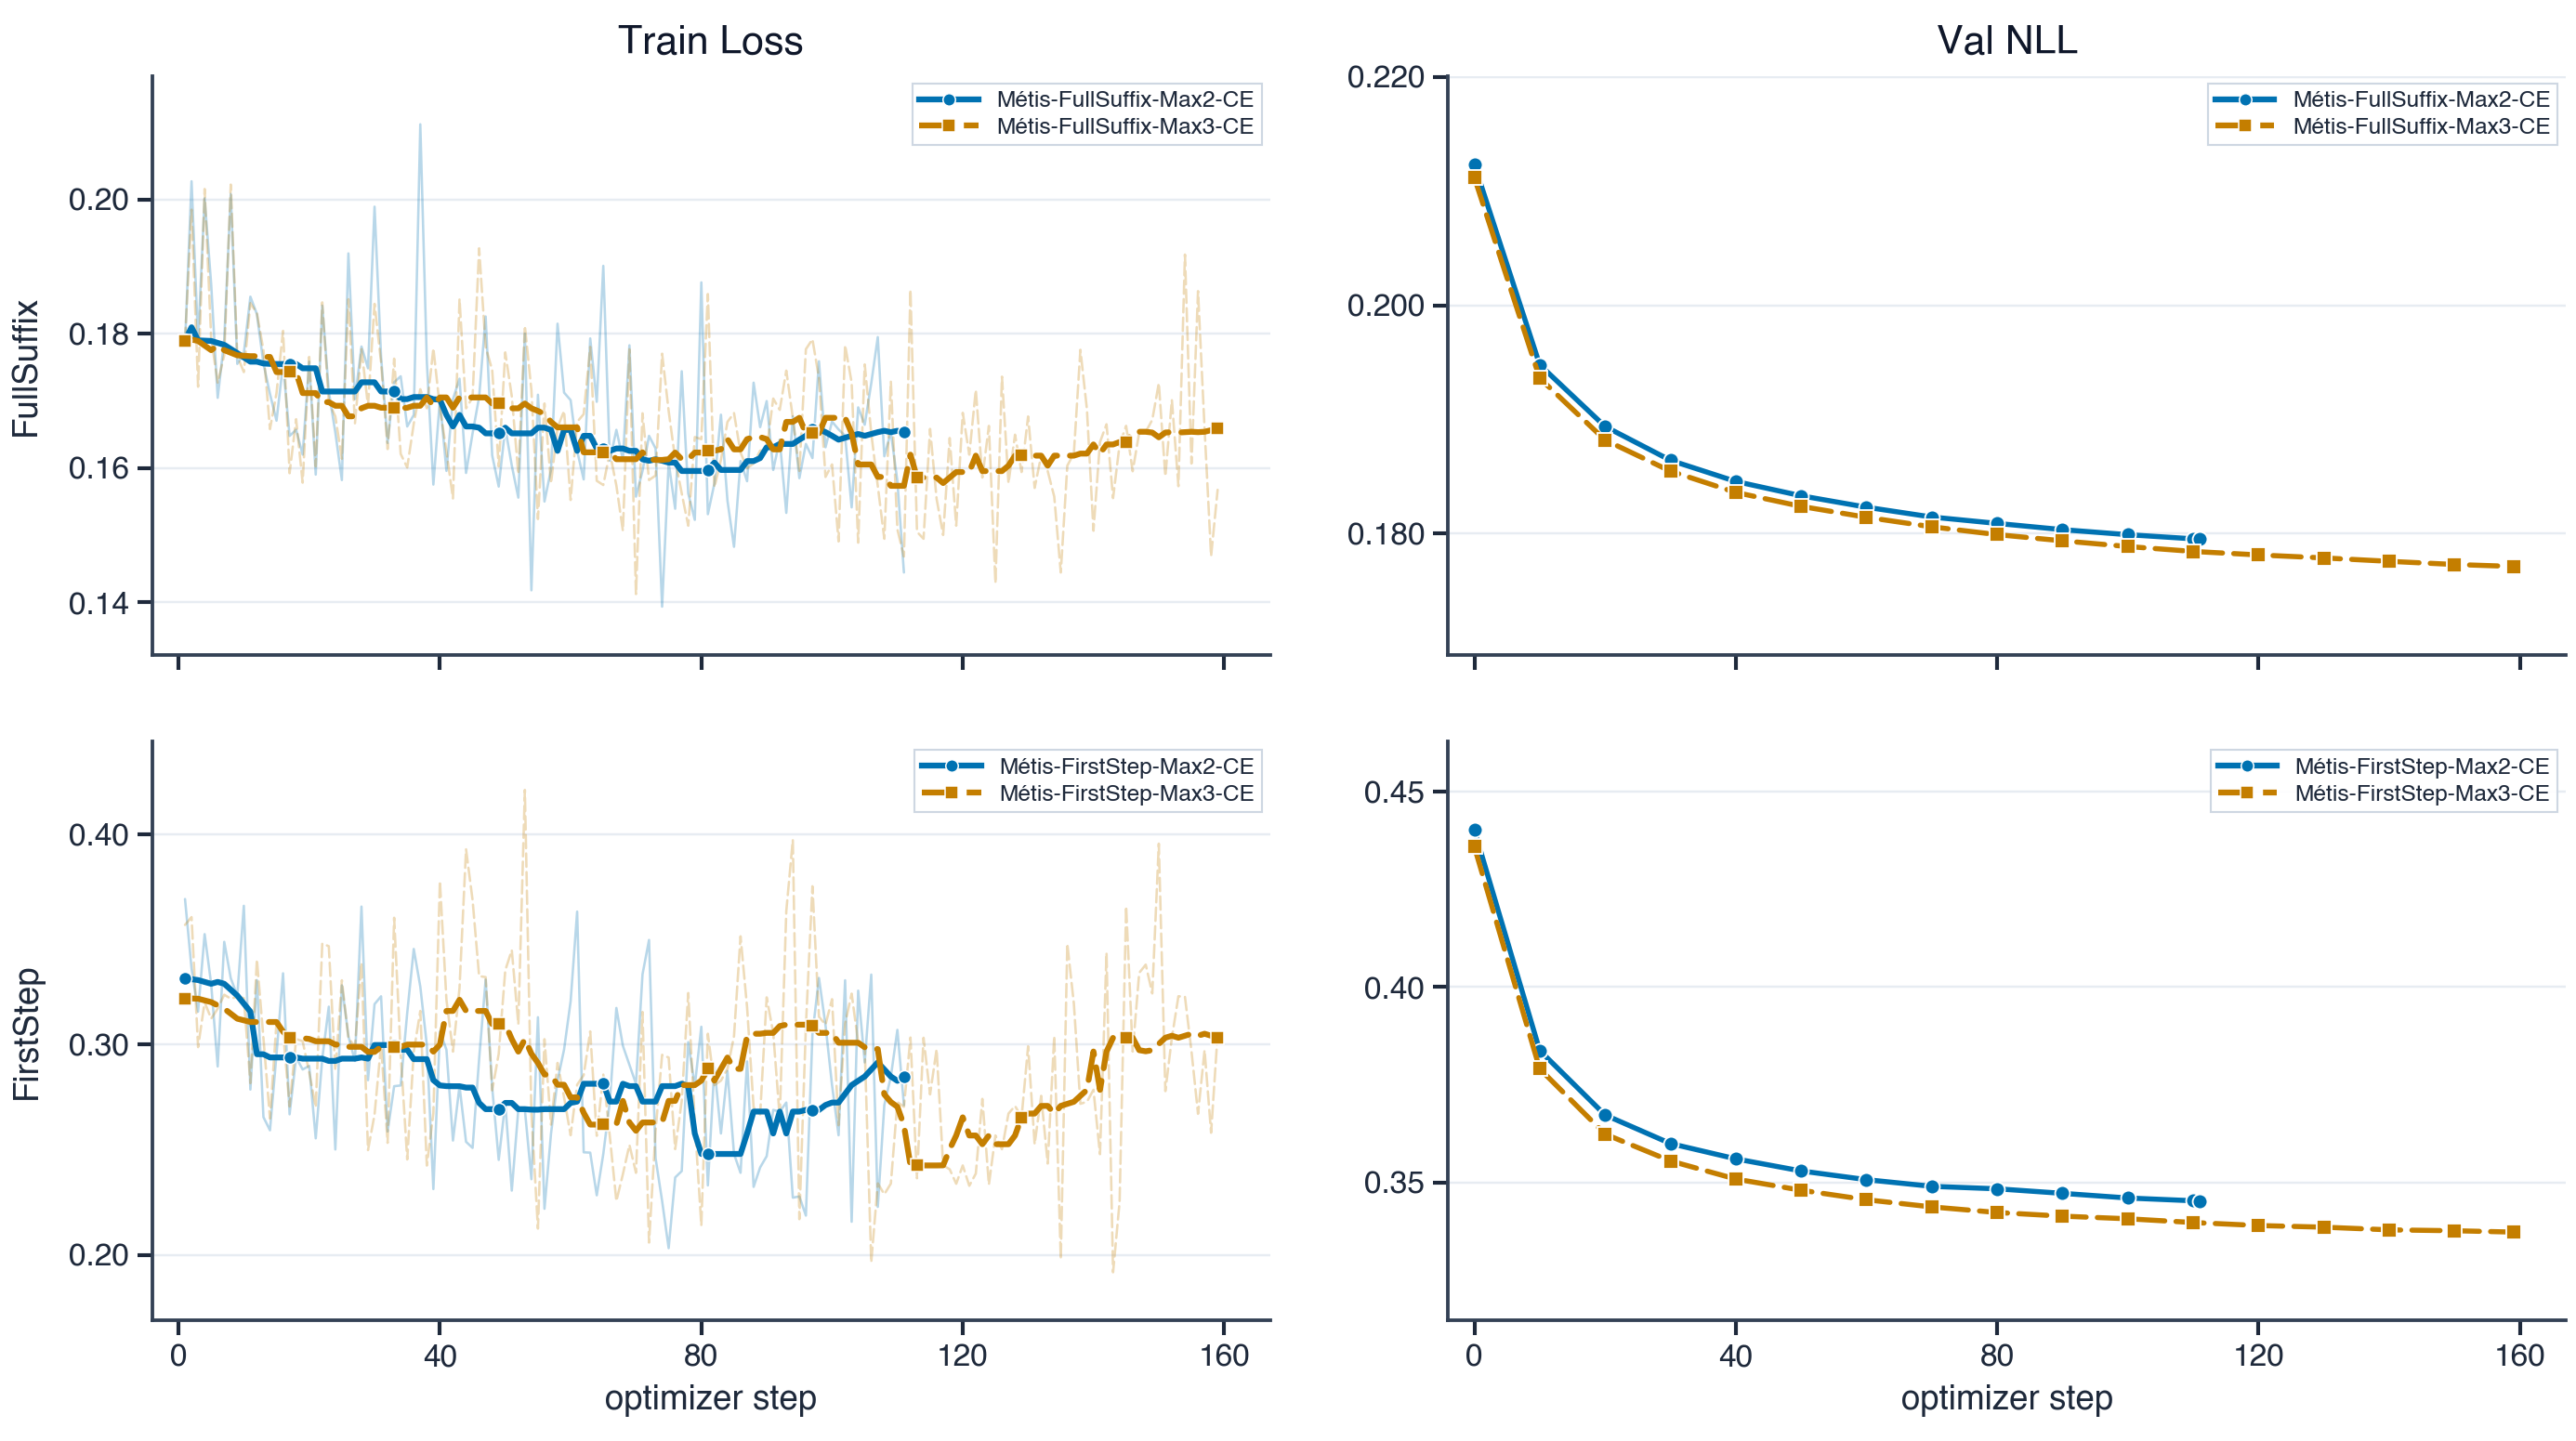
\includegraphics[width=\linewidth]
      {figures/application/metis_ce_training_logs.png}
    \\(a) CE objective
  \end{minipage}\hfill
  \begin{minipage}[t]{0.49\linewidth}
    \centering
    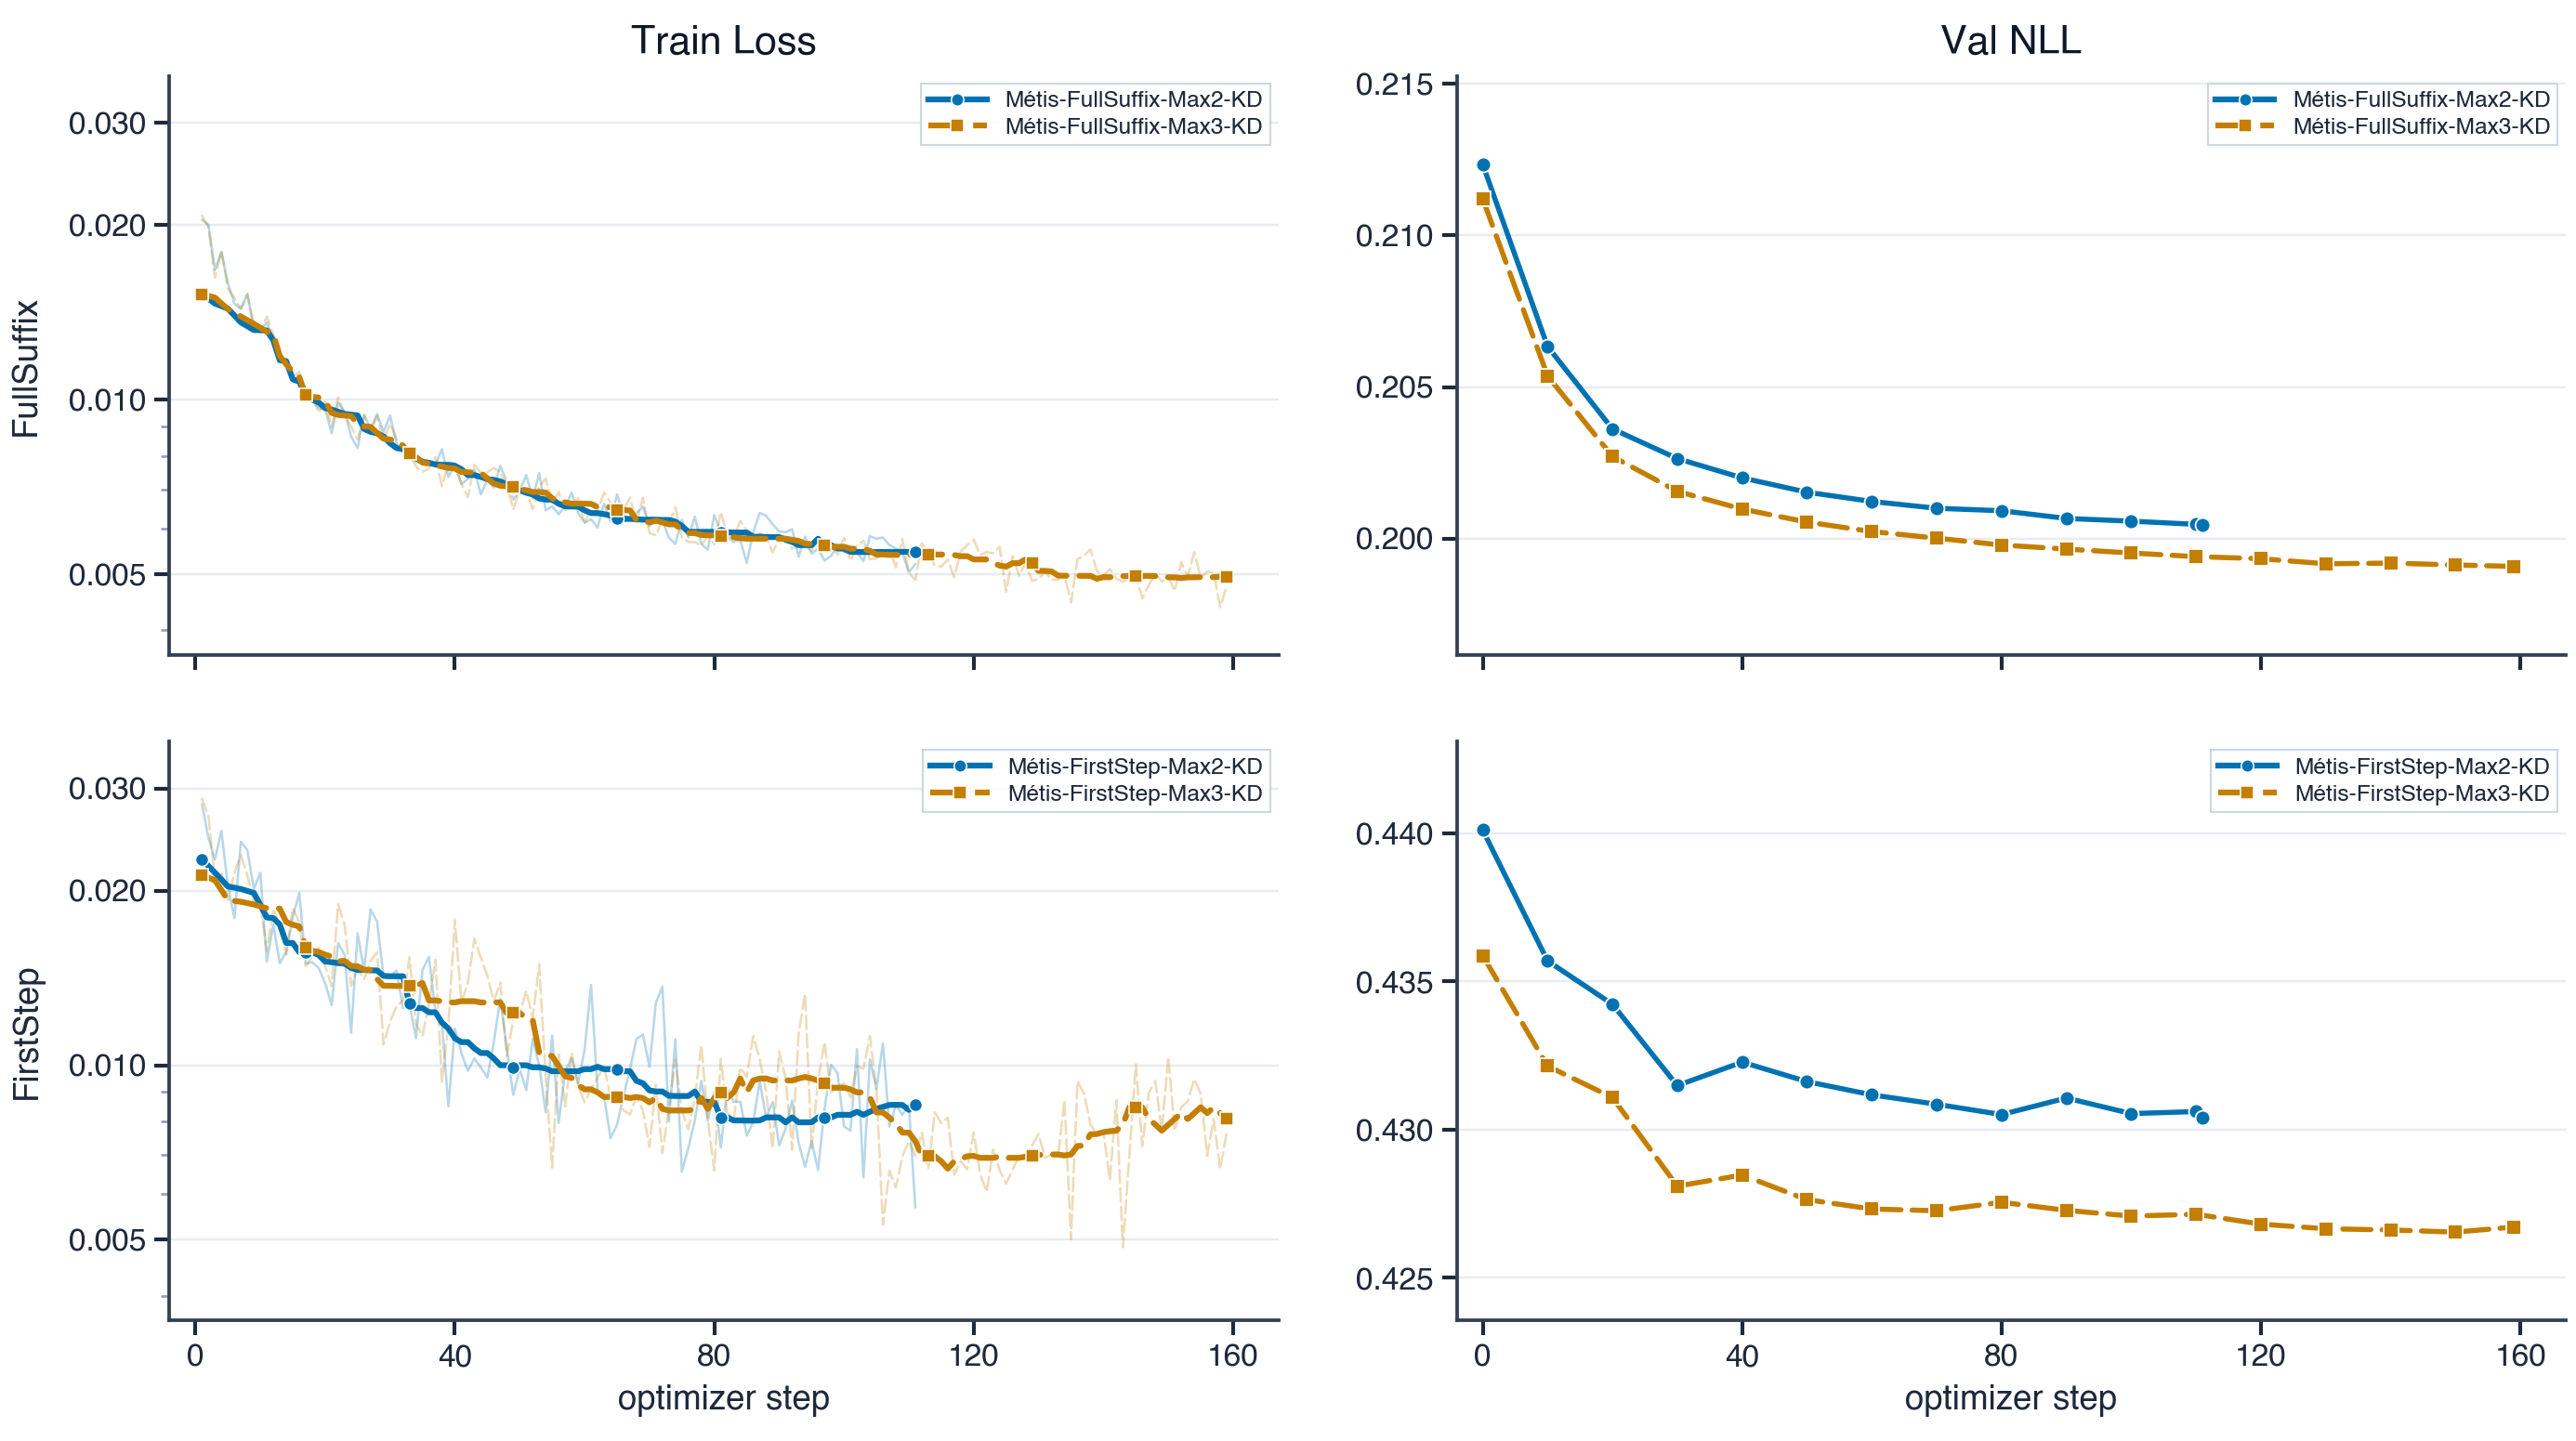
\includegraphics[width=\linewidth]
      {figures/application/metis_kd_training_logs.png}
    \\(b) KD objective
  \end{minipage}
  \caption{Training loss and validation NLL under CE and KD objectives.
  Within each panel, the left and right columns show training loss and validation NLL, respectively.
  Solid blue curves denote Max-2, and dashed orange curves denote Max-3.}
  \label{fig:training-logs}
\end{figure}

\paragraph{Optimization and Validation Behavior.}
Figure~\ref{fig:training-logs} shows decreasing validation NLL
under both objectives, with most of the reduction occurring
within the first 40 optimizer steps.
CE achieves lower final validation NLL than KD in all four
paired configurations
(Table~\ref{tab:ce-kd-diagnostics}).
For Full-Suffix-Max2, CE reduces body-token NLL from 0.2925
to 0.1866, compared with 0.2910 under KD.
The same pattern holds for tool-call tokens
(0.0603 to 0.0461 under CE versus 0.0545 under KD)
and reasoning tokens
(0.5033 to 0.4555 versus 0.4749).

\paragraph{Relation to Agent Performance.}
KD achieves higher average success rates than CE despite its
higher validation NLL (Table~\ref{tab:ce-kd-diagnostics}).
For example, Full-Suffix-Max2 records a preliminary success
rate of 37.5\% under CE, compared with 54.3\% under KD,
while its validation NLL is lower under CE
(0.1795 versus 0.2005).
The other three configurations exhibit the same qualitative
pattern. These results motivate
our selection of KD for all subsequent agent evaluations
and ablations. We use validation NLL to monitor optimization,
while selecting among KD configurations through repeated
agent executions.

\begin{table}
  \centering
  \small
  \caption{Validation NLL and preliminary agent performance under CE and KD.
  Average success rates are measured on the 100-task development subset of SWE-bench Verified
  with three runs per task. Validation NLL uses hard-label targets; lower is better.}
  \label{tab:ce-kd-diagnostics}
  \begin{tabular}{lrrrr}
    \toprule
    & \multicolumn{2}{c}{Validation NLL}
    & \multicolumn{2}{c}{Avg. Success (\%)} \\
    \cmidrule(lr){2-3}
    \cmidrule(lr){4-5}
    Configuration & CE & KD & CE & KD \\
    \midrule
    First-Step-Max2  & 0.3452 & 0.4304 & 12.5 & 52.0 \\
    First-Step-Max3  & 0.3373 & 0.4267 & 34.1 & 52.0 \\
    Full-Suffix-Max2 & 0.1795 & 0.2005 & 37.5 & 54.3 \\
    Full-Suffix-Max3 & 0.1771 & 0.1996 & 22.7 & 52.7 \\
    \bottomrule
  \end{tabular}
\end{table}



\subsection{Additional Results}
\subsubsection{Training Configuration Comparison}

\paragraph{Training Configurations.}
In Table~\ref{tab:v1_training_configurations}, we compare four Metis KD configurations
on the 100-task development subset of SWE-bench Verified under the Before Execution setting, with three runs per task. This subset is included in the full 500-task SWE-bench Verified evaluation reported in the main text.
Full-Suffix-Max2 achieves the highest average success and ties for the
highest pass@3 and pass\textasciicircum{}3, motivating its selection for full-benchmark
Metis evaluations. 

\begin{table}[tb]
  \centering
  \small
  \caption{Metis KD configurations on the 100-task development subset of SWE-bench Verified under Before Execution.
  All values are percentages; bold values indicate the highest scores in each column.}
  \label{tab:v1_training_configurations}
  \begin{tabular}{lrrr}
    \toprule
    Configuration & Avg. Success & pass@3 & pass\textasciicircum{}3 \\
    \midrule
    First-Step-Max2  & 52.00 & 65.00 & 38.00 \\
    First-Step-Max3  & 52.00 & 61.00 & \textbf{42.00} \\
    Full-Suffix-Max2 & \textbf{54.33} & \textbf{66.00} & \textbf{42.00} \\
    Full-Suffix-Max3 & 52.67 & \textbf{66.00} & 36.00 \\
    \bottomrule
  \end{tabular}
\end{table}

\paragraph{Full-Benchmark Comparison.}
In Figure~\ref{fig:swe_versions}, we compare Metis and MemT-1.0-Nano with the backbone and textual-experience baselines on SWE-bench Verified (500 tasks) and SWE-bench Multilingual (300 tasks). Both memory models improve average success and pass\textasciicircum{}3 over the backbone. Relative to Metis, MemT-1.0-Nano has higher pass@3 but lower pass\textasciicircum{}3 in all four settings. 

\begin{figure*}[t]
  \centering
  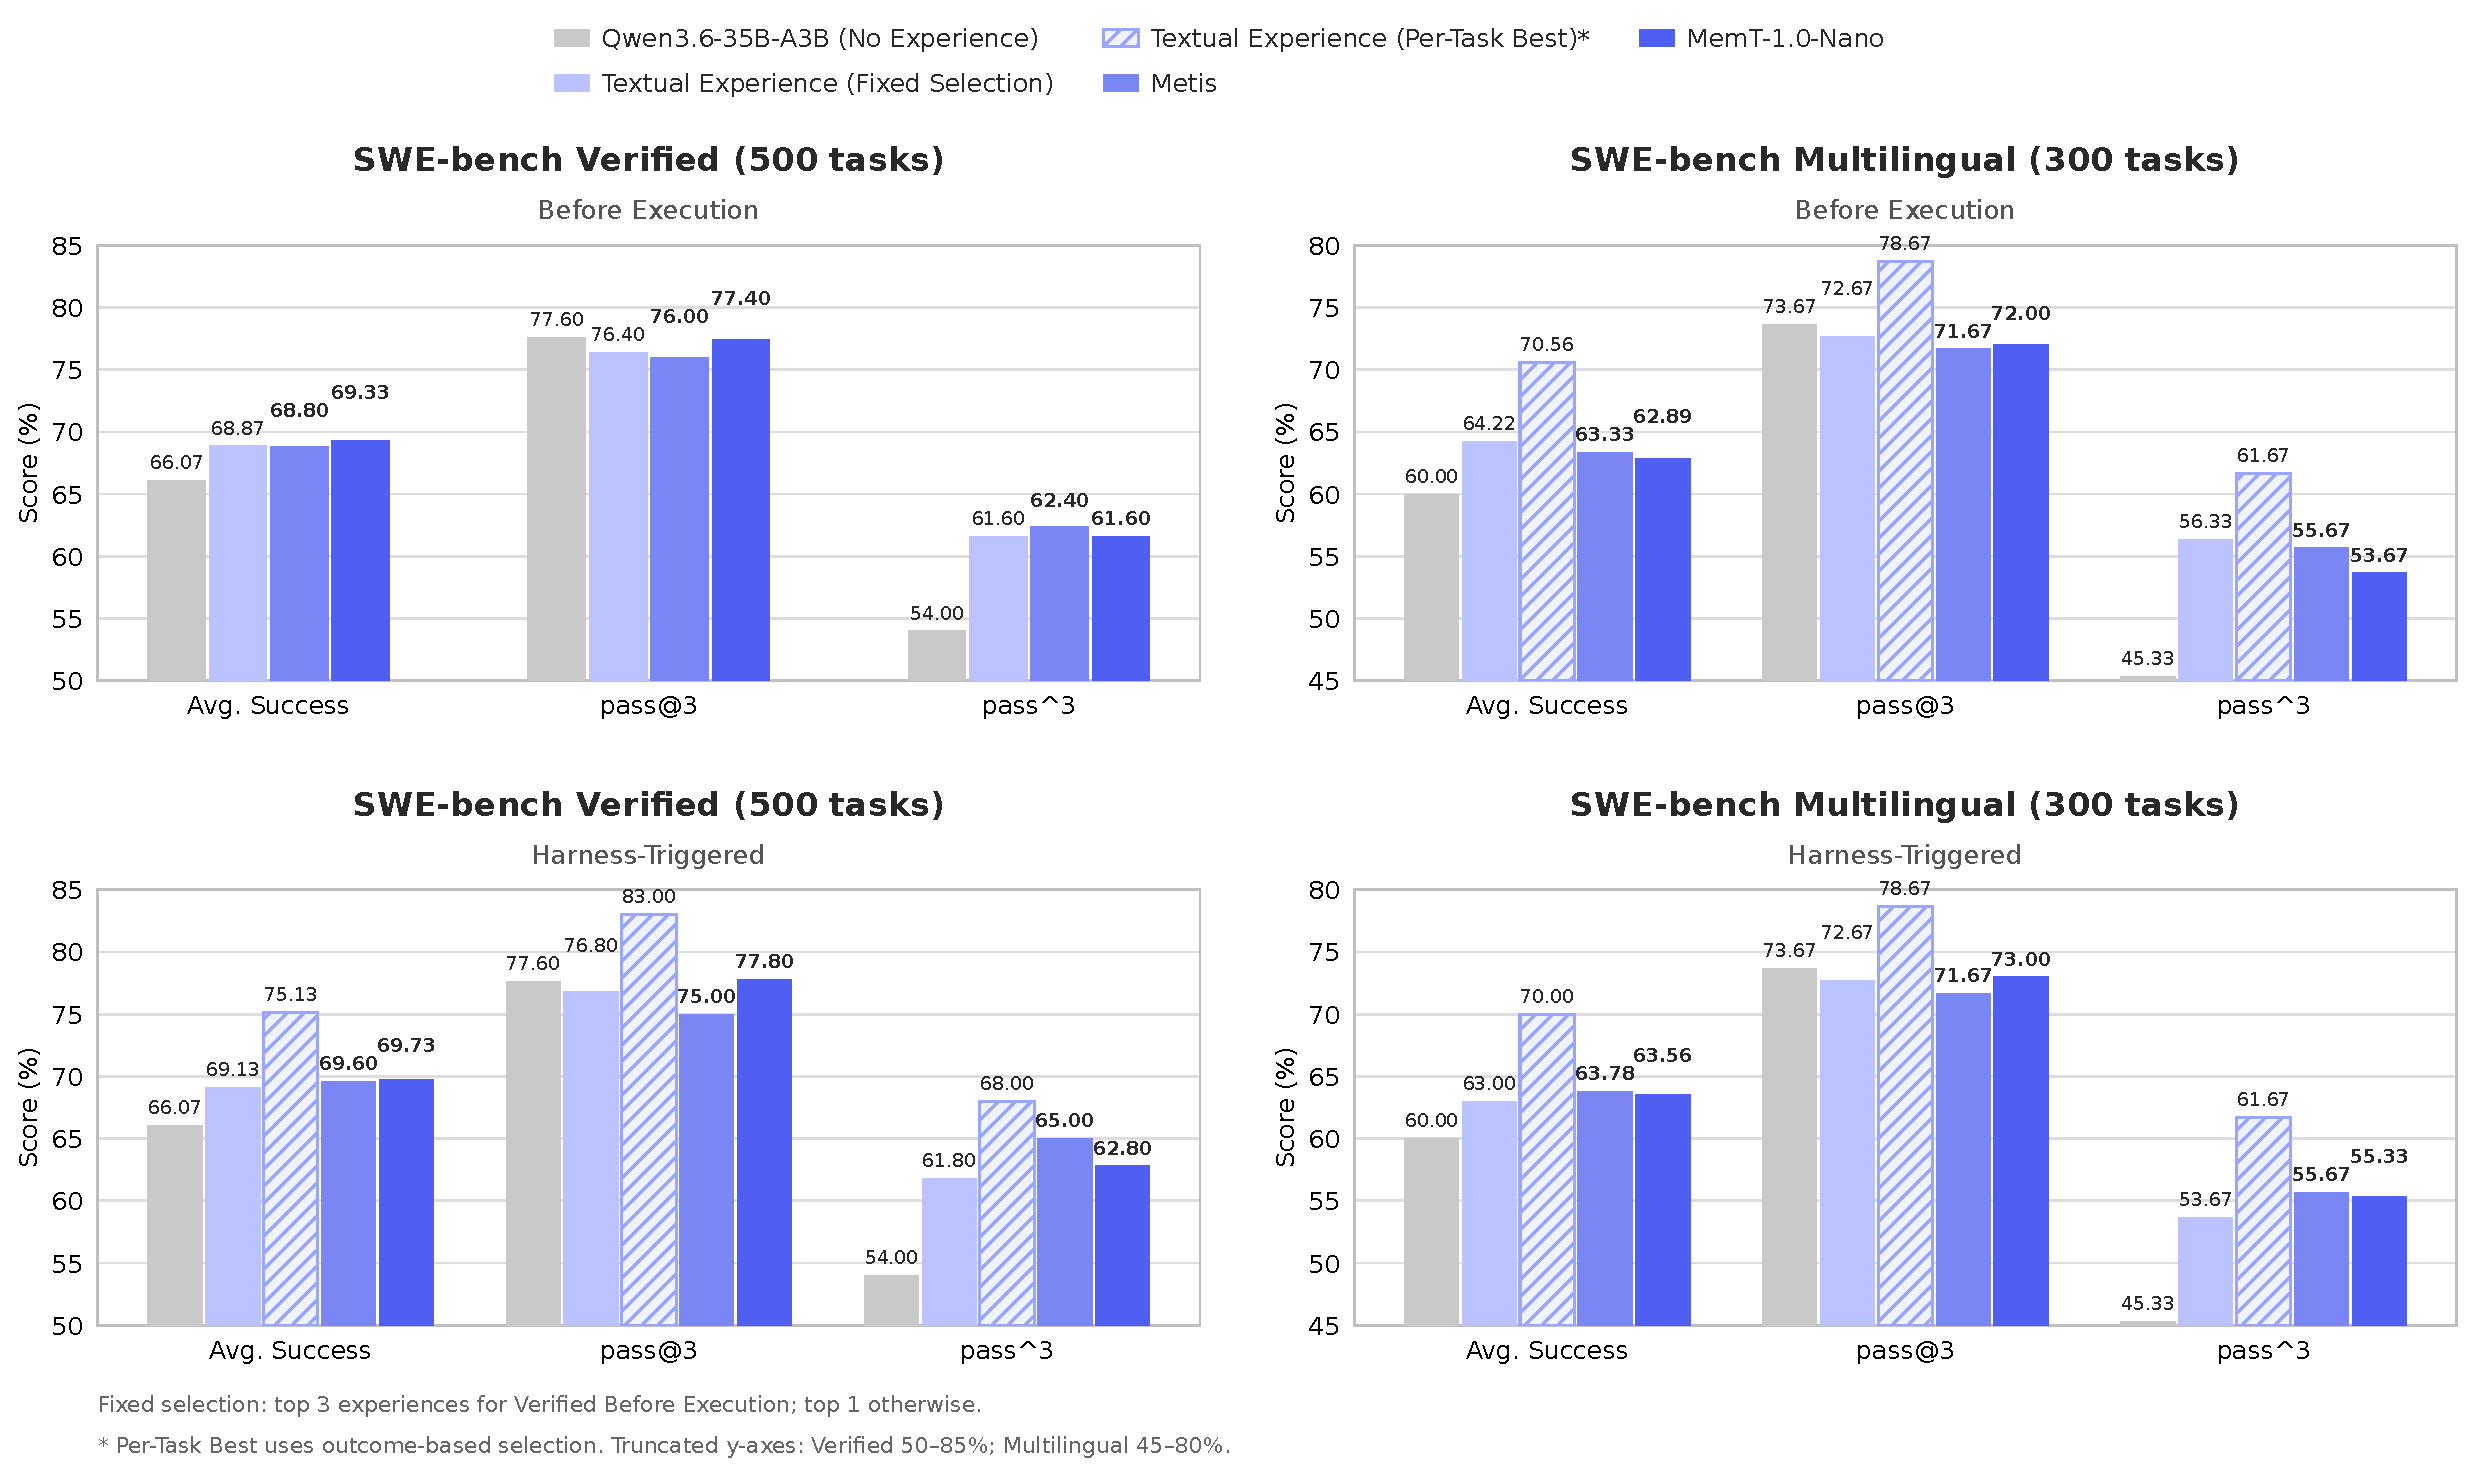
\includegraphics[width=\textwidth]{figures/application/fig_swe_v1_v2_combined.pdf}
  \caption{Agentic coding performance on SWE-bench Verified and SWE-bench Multilingual under
  Before Execution (top) and Harness-Triggered (bottom). Each task is evaluated in three runs.}
  \label{fig:swe_versions}
\end{figure*}



\subsubsection{Experience Selection}

We compare Textual Experience selection strategies on SWE-bench Multilingual (Table~\ref{tab:selection_multilingual}). Fixed Rank-$k$ uses the single experience at retrieval rank $k$. Per-Task Best selects among three candidates by the number of successful runs, breaking ties by retrieval rank. Since the same runs are used for selection and reporting, it serves as an outcome-selected reference. Rank-1 achieves the highest average success under Before Execution, whereas Rank-2 performs best under Harness-Triggered. Per-Task Best outperforms the fixed-rank strategies in both settings, suggesting that improved experience selection could further benefit task performance.

\begin{table}[tb]
  \centering
  \small
  \caption{Textual Experience selection on SWE-bench Multilingual (300 tasks).
  Fixed Rank-$k$ uses the single experience at rank $k$; Per-Task Best selects among three candidates
  using evaluation outcomes. All values are percentages.}
  \label{tab:selection_multilingual}
  \begin{tabular}{lrrr}
    \toprule
    Method & Avg. Success & pass@3 & pass\textasciicircum{}3 \\
    \midrule
    \multicolumn{4}{l}{\textit{Before Execution}} \\
    No Experience                   & 60.00 & 73.67 & 45.33 \\
    Textual Experience: Fixed Rank-1             & 64.22 & 72.67 & 56.33 \\
    Textual Experience: Fixed Rank-2             & 61.89 & 72.67 & 51.33 \\
    Textual Experience: Fixed Rank-3             & 63.78 & 74.00 & 54.33 \\
    Textual Experience: Per-Task Best           & 70.56 & 78.67 & 61.67 \\
    \midrule
    \multicolumn{4}{l}{\textit{Harness-Triggered}} \\
    No Experience                   & 60.00 & 73.67 & 45.33 \\
    Textual Experience: Fixed Rank-1             & 63.00 & 72.67 & 53.67 \\
    Textual Experience: Fixed Rank-2             & 64.44 & 72.00 & 56.67 \\
    Textual Experience: Fixed Rank-3             & 63.56 & 72.00 & 54.67 \\
    Textual Experience: Per-Task Best           & 70.00 & 78.67 & 61.67 \\
    \bottomrule
  \end{tabular}
\end{table}

